\documentclass{standalone}
\usepackage{tikz}
\usetikzlibrary{shapes,arrows,positioning,automata}

\begin{document}
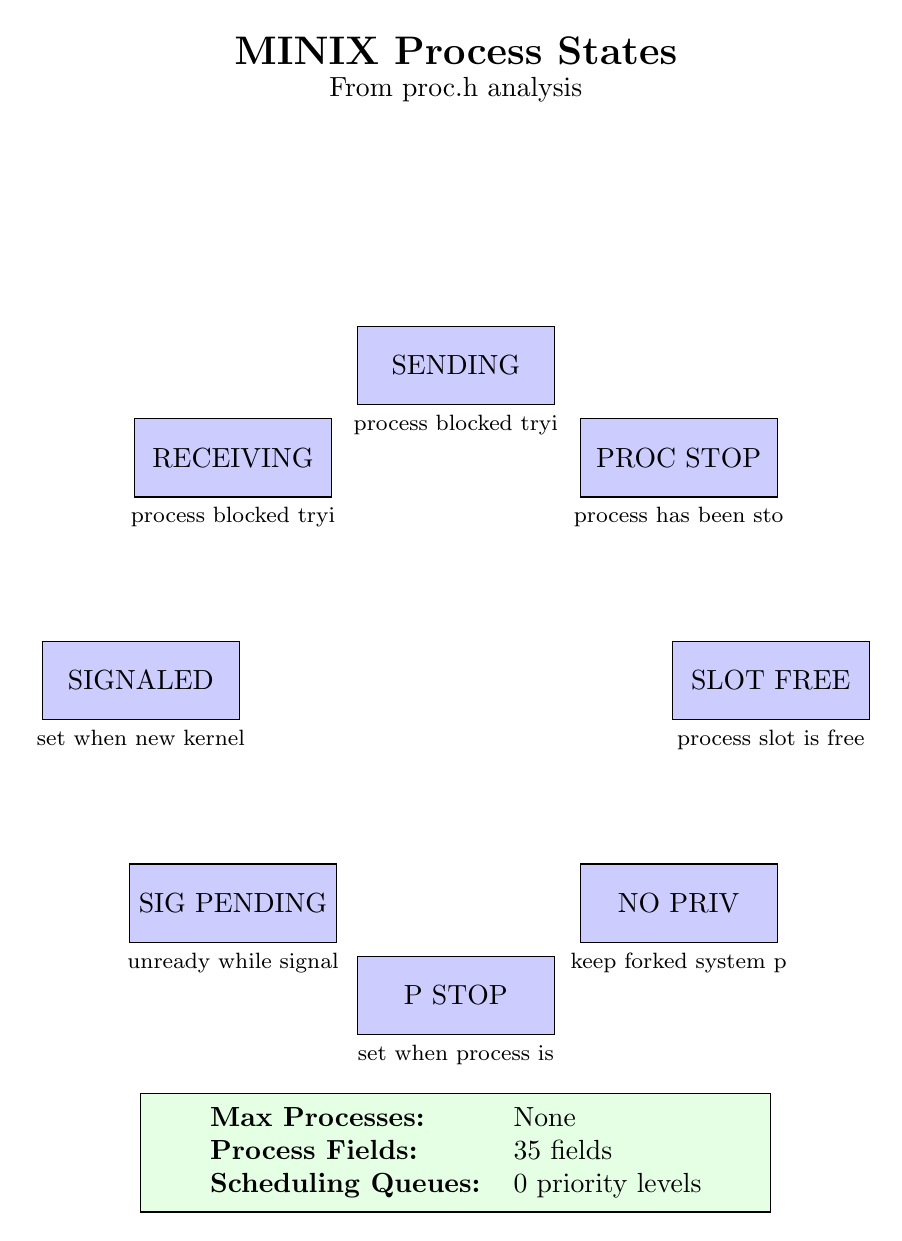
\begin{tikzpicture}[
    state/.style={rectangle, draw=black, fill=blue!20, minimum width=2.5cm, minimum height=1cm},
    arrow/.style={->, >=stealth, thick}
]

% Title
\node[font=\Large\bfseries] at (0, 8) {MINIX Process States};
\node[font=\normalsize] at (0, 7.5) {From proc.h analysis};

\node[state] (s0) at (4.00, 0.00) {SLOT FREE};
\node[font=\footnotesize, below] at (s0.south) {process slot is free};

\node[state] (s1) at (2.83, 2.83) {PROC STOP};
\node[font=\footnotesize, below] at (s1.south) {process has been sto};

\node[state] (s2) at (0.00, 4.00) {SENDING};
\node[font=\footnotesize, below] at (s2.south) {process blocked tryi};

\node[state] (s3) at (-2.83, 2.83) {RECEIVING};
\node[font=\footnotesize, below] at (s3.south) {process blocked tryi};

\node[state] (s4) at (-4.00, 0.00) {SIGNALED};
\node[font=\footnotesize, below] at (s4.south) {set when new kernel };

\node[state] (s5) at (-2.83, -2.83) {SIG PENDING};
\node[font=\footnotesize, below] at (s5.south) {unready while signal};

\node[state] (s6) at (-0.00, -4.00) {P STOP};
\node[font=\footnotesize, below] at (s6.south) {set when process is };

\node[state] (s7) at (2.83, -2.83) {NO PRIV};
\node[font=\footnotesize, below] at (s7.south) {keep forked system p};


% Process Table Info
\node[draw=black, fill=green!10, minimum width=8cm] at (0, -6) {
\begin{tabular}{ll}
\textbf{Max Processes:} & None \\
\textbf{Process Fields:} & 35 fields \\
\textbf{Scheduling Queues:} & 0 priority levels
\end{tabular}
};

\end{tikzpicture}
\end{document}